\chapter{緒言}
\labsec{introduction}
\section{研究背景および目的}
\labsec{background}
\label{緒言}
近年,複数の移動ロボットから構成される群ロボットシステム(Swarm Robotic Systems)の研究が進められている~\cite{multiRobotCoodination}.複数のロボットが協調して行動することにより,単一のロボットだけでは達成できないような作業を行ったり,より効率的に作業を処理したりすることが可能となる~\cite{swarm}.群ロボットには頑強性(robustness),柔軟性(flexibility),拡張性(scalability)という特徴が求められる.これらの特徴の意味は次のように書ける~\cite{swarmBehaviour}.
\begin{itemize}
 \item 頑強性:群の一部の個体が欠落しても群れ全体の機能を損なわない
 \item 柔軟性:環境が変化したりタスクが変更になったとしてもそれらに適応してタスクを遂行できる
 \item 拡張性:群れの規模が大きくなっても群れ全体の機能が破綻しない
\end{itemize}
これらの特徴を活かした群ロボットのタスクとして,環境センシングやモニタリング~\cite{sensing,monitoring},物体搬送~\cite{motionPlanning}などがあり,さまざまな研究が進められている~\cite{mrs}.その中で,本研究では群ロボットによる協調運搬に着目する.

群ロボットの協調運搬の方式は掴む方法~\cite{grasp1,grasp2,grasp3,swarmBot},押す方法~\cite{push-only1,push-only2,push-only3,argos},囲む方法~\cite{caging1,caging2,caging3}の大きく3つに分類される.
掴む方法を使用する研究として,Dorigoらの「Swarm-bots」と呼ばれるロボット群がある.各ロボットに2本指で挟むグリッパの把持機構が搭載されている.対象物体を認識し,把持機構をうまく操ることで力の相互作用による協調運搬を実現している~\cite{swarmBot}.
また,押す方法を使用する研究として,藤澤らの「ARGOS01」と呼ばれる把持機構なしのゴールや物体を認識できるロボット群がある.蟻の群行動模したフェロモン・コミュニケーションによる他個体誘引および押すことによる餌を蟻の巣に模した場所までの協調運搬を実現している~\cite{argos}.
そして,囲む方法を使用する研究として,WangらのLeader-Follower型のアルゴリズムに基づく制御を行う群ロボットがある.Leader-Follower型の制御系とは移動ロボット群のうち1台をLeader,残りをFollowerと区別し機能分化されたものである.この研究ではLeaderロボットのみに移動軌跡を与え物体を押す.一方,物体を囲むFollowerロボットが物体からの反力・モーメントに基づきその移動軌跡を推定し,協調運搬を実現している~\cite{caging1}.
このうち掴む方法は押す方法と囲む方法と比べて対象物体を2本指で挟むグリッパなどの機構によって掴むことでより安定に協調運搬を実現できる.しかし,対象物体を認識し判断すること,それに合わせた把持動作を考慮すること,把持状態の維持することなどを行うための制御が必要である.
さらに,物体の形によって把持機構ごとに得意不得意が分かれるので,あらゆる形状の物体の把持には至っていない.
それに対して,押す方法と囲む方法は,複雑な把持機構なしで協調運搬を実現できる.
しかし,従来の押す方法と囲む方法には未解決の課題がある.それは倒れやすい不安定な物体の運搬である.

そこで,ロボットが積み上がることで対象物体の重心付近を支持可能な群ロボットシステムは,複雑な把持機構なしで倒れやすい不安定な物体を運搬する良い解決案になるのではないかと考えた.
これを実現するために,ロボット群を対象物体を支持する支持部と全体を移動する移動部に適宜に入れ替われる.対象物体の重心付近を支持するために,支持部は他のロボットに乗り上げられるようなロボットを提案する.すなわち,ロボットが積み上がることより,重心が高い不安定な物体でも支持することができると考えられる.しかし,ロボットの台数に制限があるため,支持部のロボット台数が多いほどより安定な運搬が行うことができる.その一方で,移動部の台数が少なくなり,移動部のロボットに大きな負担をかけるため,協調運搬の効率が悪くなる.したがって,効率よく協調運搬する群ロボットシステムを実現するために,物体の形や運搬速度などの条件に応じて,移動部と支持部の割合を適切に設計することが望ましい.

よって,本研究では,\reffig{proposed-system}に示すように,ロボットが対象物体の重心付近まで乗り上げることにより,ロボット自身の体を活用して物体を支持し,あらゆる形状の物体の協調運搬を実現する群ロボットシステムを提案する.
\begin{figure}[tb]
  \centering
  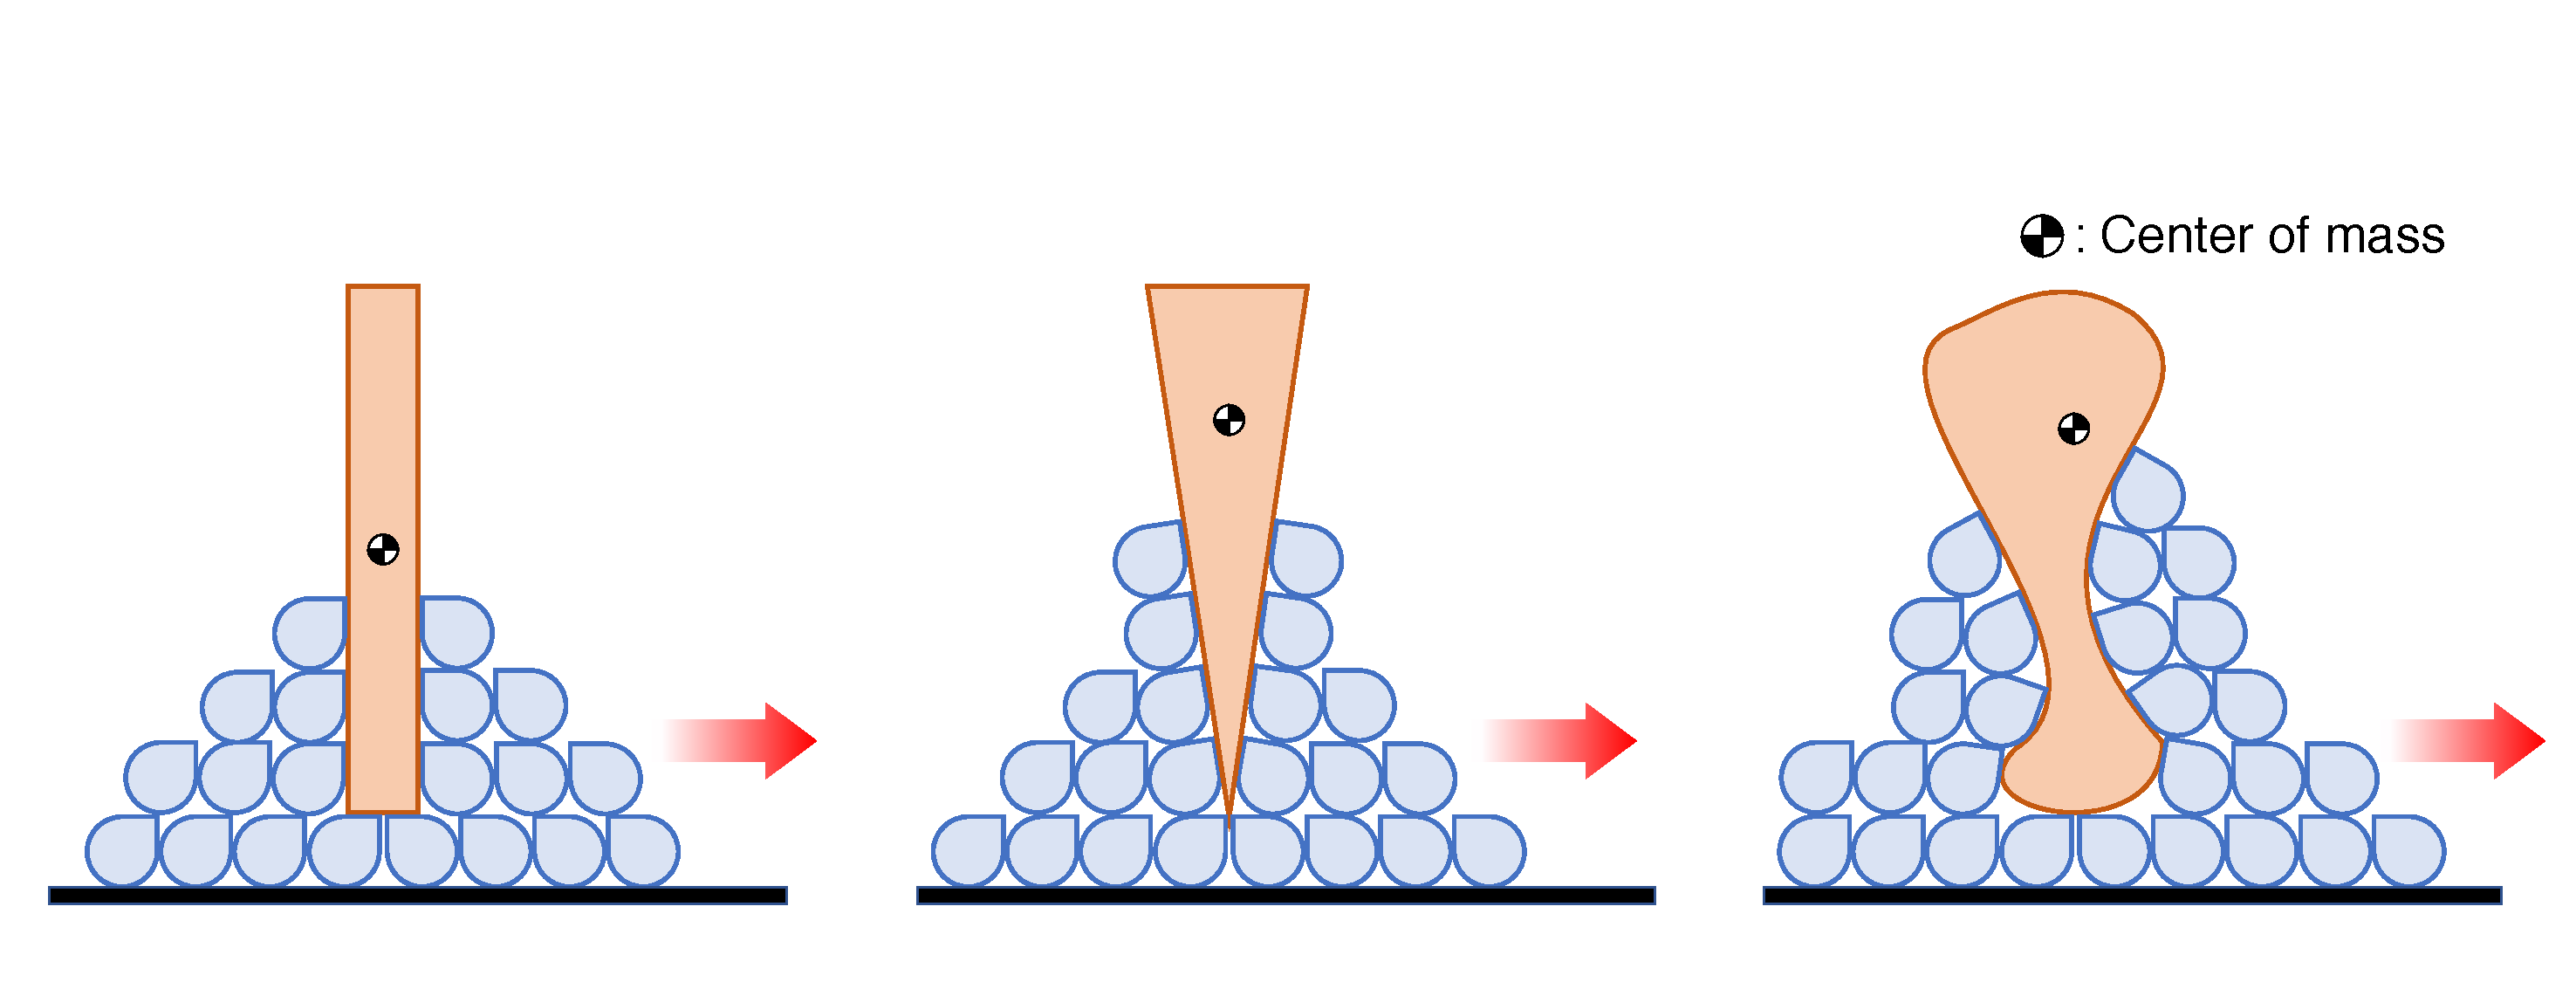
\includegraphics[width=0.96\columnwidth]{figure/proposed-system.pdf}
  \caption{Proposed system}
  \label{fig:proposed-system}
\end{figure}
また,\reffig{tradeoff}では,移動部と支持部の割り当てによって,物体の安定性と全体の機動性の間のトレードオフを示す.
\begin{figure}[bt]
  \vspace{0mm}
  \centering
  \begin{tabular}{c}
    \begin{minipage}[ht]{0.5\columnwidth}
      \centering
      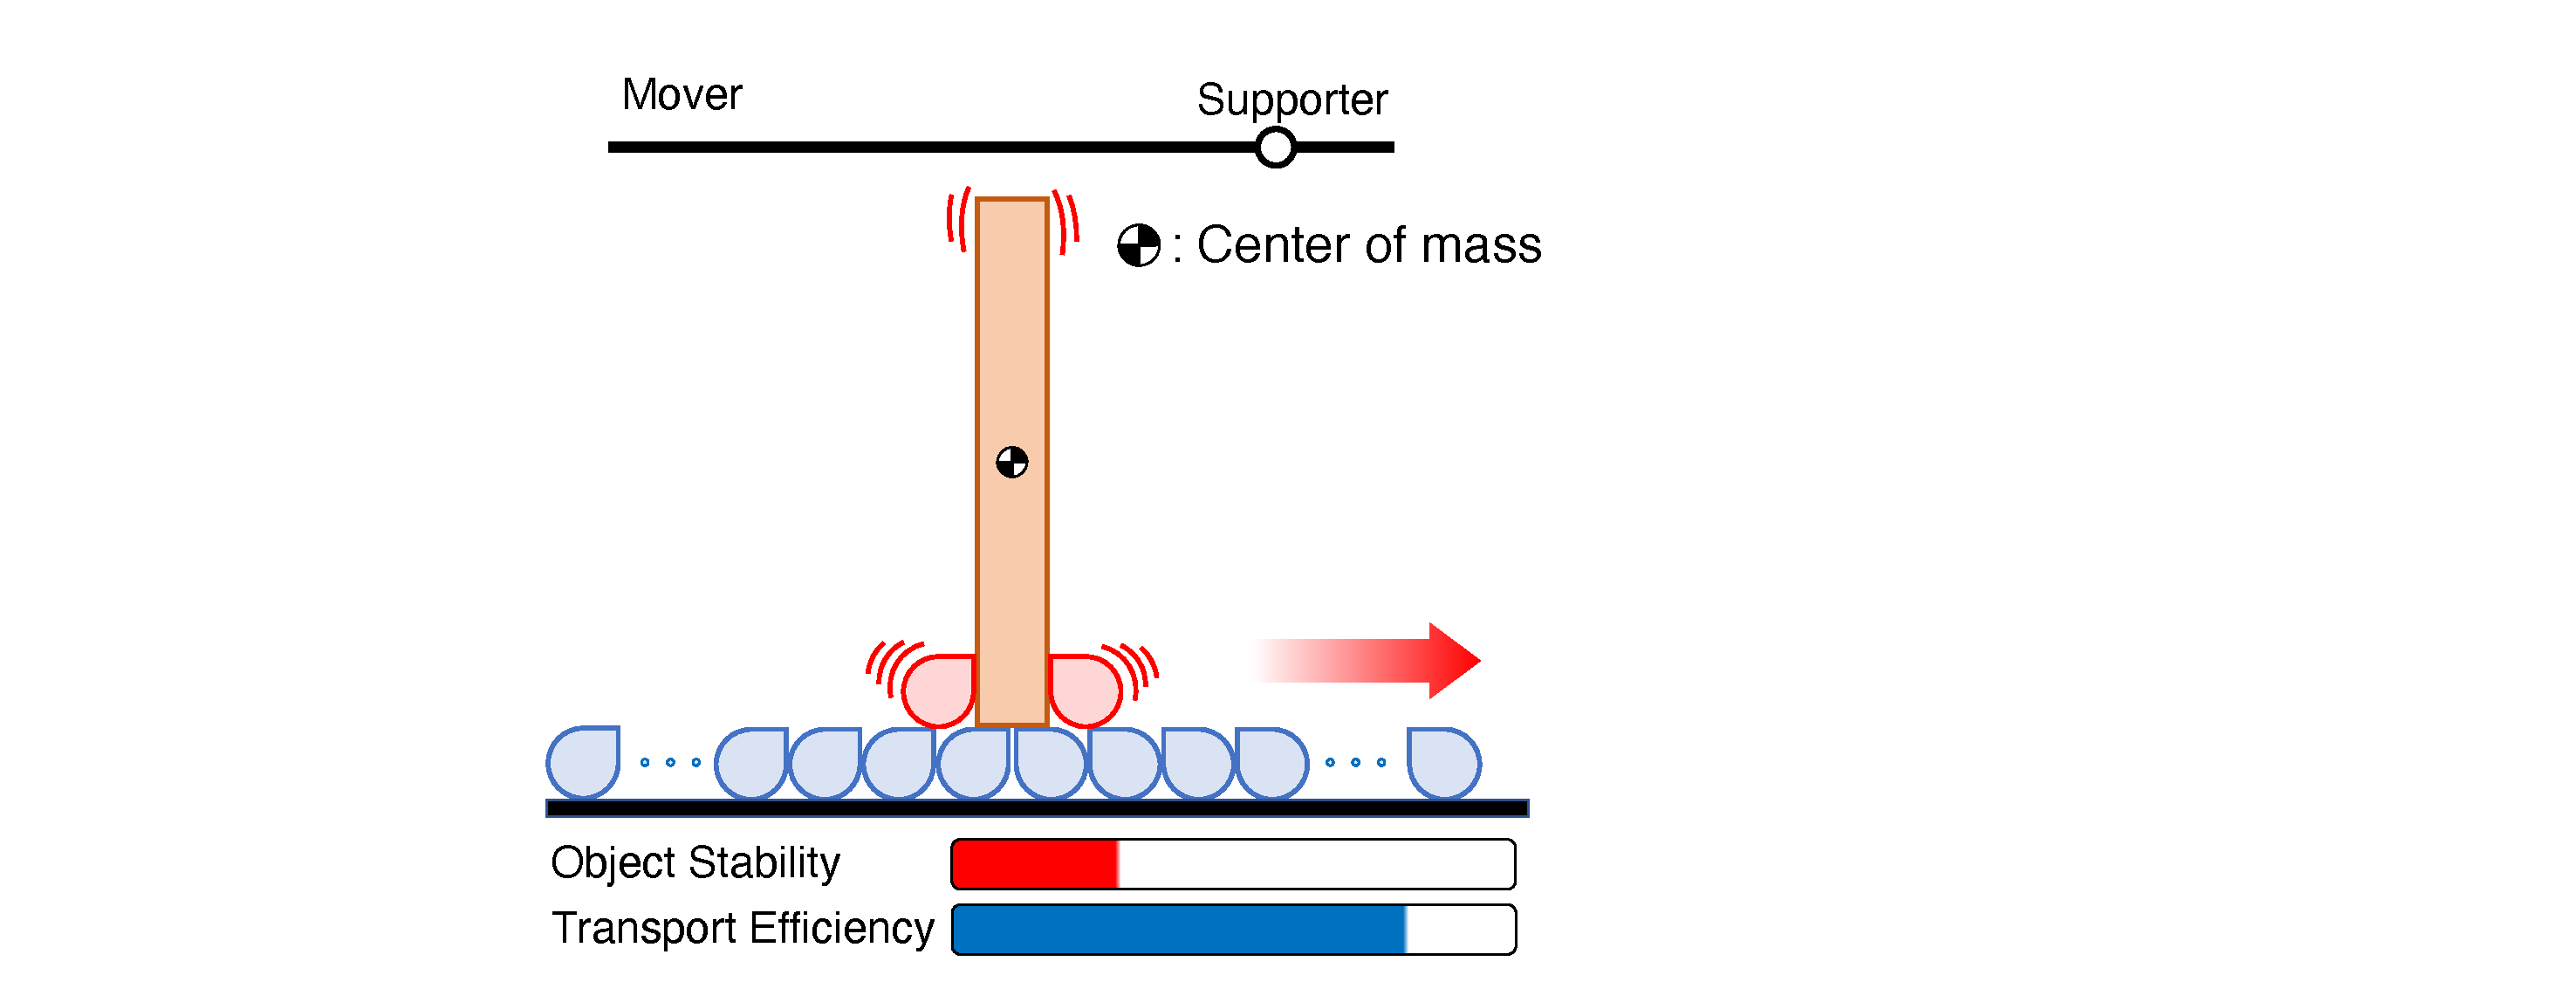
\includegraphics[trim=0 0 0 0, clip,width=\columnwidth]{figure/tradeoff-fast.pdf}
      \subcaption{Supporter: 2, Mover: 18}
      \labfig{tradeoff1}
    \end{minipage}
    \begin{minipage}[ht]{0.5\columnwidth}
      \centering
      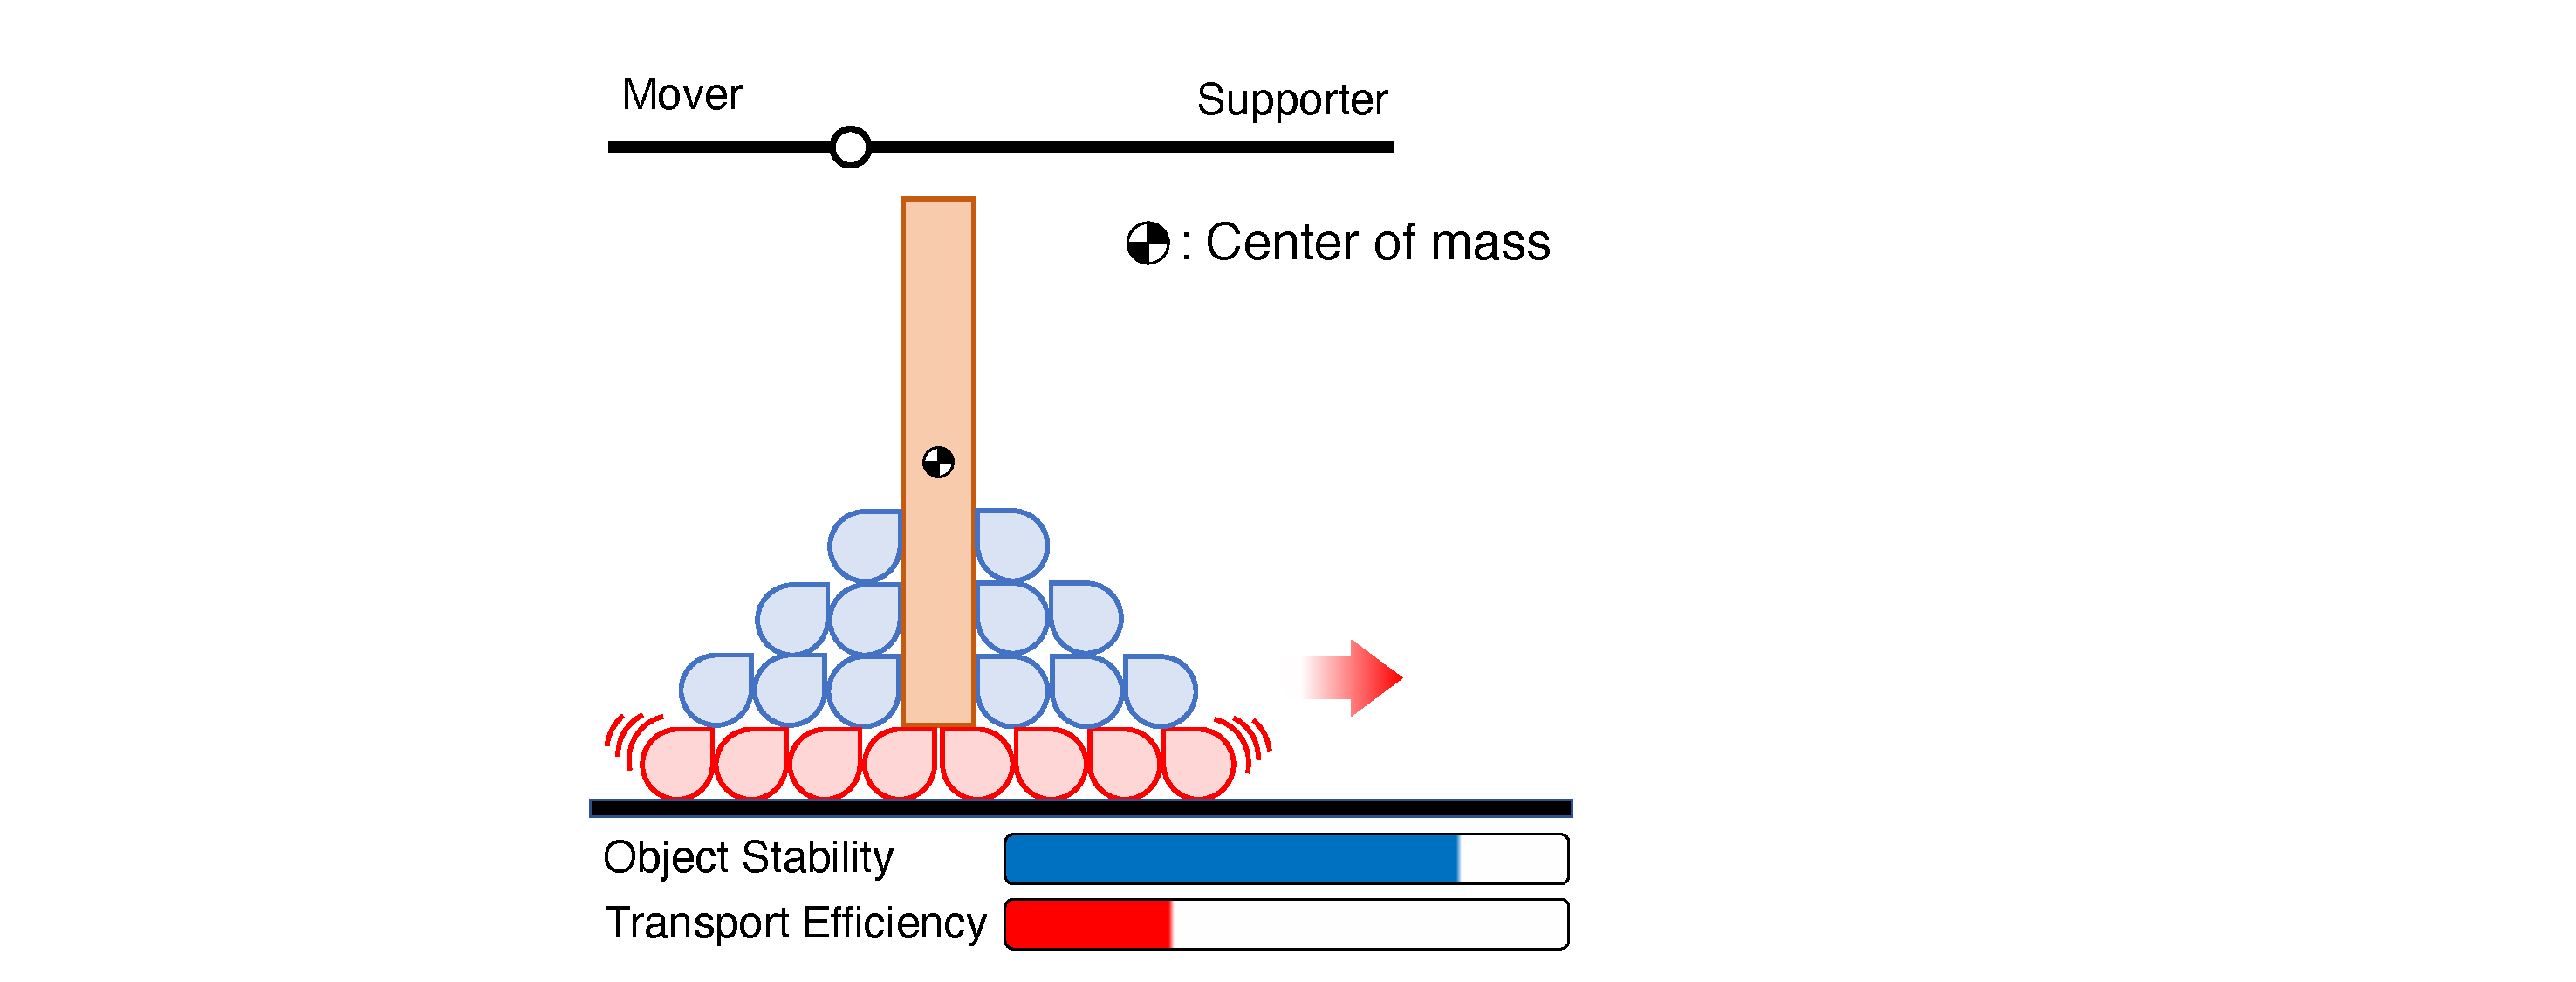
\includegraphics[trim=0 0 0 0, clip,width=\columnwidth]{figure/tradeoff-stable.pdf}
      \subcaption{Supporter: 12, Mover: 8}
      \labfig{tradeoff2}
    \end{minipage}
  \end{tabular}
  \centering
  \caption{Tradeoff between stability and mobility}
  \labfig{tradeoff}
\end{figure}
最終目標として,移動部と支持部の最適な割合を設計し,機能を適応的に分化させながら,協調して運搬作業を行うシステムの実現を目指している.すなわち,不安定物体の姿勢を安定させることと効率よく運搬することを両立させる群ロボットシステムの実現を目指している.
本研究では,その前段階として,乗り上げることで対象物体を支持でき,乗り上げたり,降りたりすることによって支持部と移動部の間で切り替えられるロボットを製作する.

それに向けて本論文では,提案システムのモデリングをして,搬送物体をロボットで支持するための条件を検討し,それをもとに実機を製作した.
また,モデリングした式からロボットと物体の高さの比を設計することに注目し,隣接しているロボットに乗り上げられるロボットを製作し,ロボットが積み上がることで,対象物体の支持が可能であることを示す.
さらに,物体の姿勢をロボットにフィードバックし,ロボットの前進力を制御することで,物体をより安定に支持できることを示す.

\section{本論文の構成}
本論文の構成は,以下の通りである.
まず,2章では提案したシステムについて述べる.
次に,3章で開発した不安定物体が支持可能な群ロボットについて述べる.
そして,4章で製作したロボットを用いて実験を行い,実験結果に対する考察について述べる.
最後に,5章で本論文をまとめる.

